%! Author = thibaultchausson
%! Date = 23/07/2023

\subsection{Sujet}\label{subsec:sujet}

Le but de ce projet audiovisuel est de réaliser des courtes vidéos, appelées Reels sur Instagram, pour montrer la diversité de l'engagement associatif, mais plus particulièrement l'engagement des étudiant·e·s.

Le projet mettra en lumière divers moments de la vie estudiantine, à travers des interviews d'étudiant·e·s, afin de promouvoir les activités dont ils·elles sont responsables au sein de l'\gls{AE} \gls{UTBM}.

L'objectif principal de ce projet est de communiquer sur les différents événements de l'\gls{AE}, ainsi que ses temps forts.
Je peux citer, de manière non exhaustive, le nouveau principe d'élection pour le Pôle Des Festivités (\gls{PDF}), les soirées d'envergure co-réalisées avec les BDE de Belfort, et encore la promotion de l'engagement dans l'association\ldots

Comme évoqué précédemment, la motivation première de ce sujet est la promotion de la vie associative estudiantine.
Je suis motivé à donner une nouvelle image de l'\gls{AE}, en montrant que derrière cette association tentaculaire, il y a des étudiant·e·s engagé·e·s pour améliorer le cadre de vie de leurs pairs.
De plus, je trouve que donner la parole aux différent·e·s instigateur·trice·s de ces changements est d'autant plus gratifiant pour eux.

\subsection{Méthodes}\label{subsec:methodes}

\subsubsection{Le fond}

Comme évoqué auparavant, mon objectif est de promouvoir l'engagement associatif, en particulier au sein de l'\gls{AE} de l'\gls{UTBM}.
Pour atteindre cet objectif, je compte mettre en avant les membres actif·ve·s de cette association, afin de montrer leur implication exemplaire dans divers domaines de cette grande association.

En d'autres termes, je souhaite susciter chez les autres étudiant·e·s l'envie de s'impliquer, en leur montrant que la vie associative de l'\gls{UTBM} est riche et dynamique.

\subsubsection{La forme}

Pour mener à bien ce projet, j'ai décidé de réaliser de courtes capsules vidéo dynamiques d'une durée de 1 à 1 minute 30, afin de maintenir l'attention de mon audience sur le message que je souhaite transmettre.
De ce fait, le format des Reels Instagram\footnote{Un Reel est une vidéo courte et divertissante de moins de 90 secondes (\href{https://about.instagram.com/fr-fr/features/reels}{Reels Instagram}).} s'adapte parfaitement à ces contraintes.

Les plateformes numériques de communication en réseau ont révolutionné notre manière de communiquer, d'obtenir des informations et de nous divertir ; elles ont eu un impact considérable sur les nouvelles générations.
L'utilisation des réseaux sociaux a connu une croissance exponentielle avec la pandémie de COVID-19, en partie à cause des différents confinements.
L'activité des nouvelles générations sur TikTok et Instagram a modifié les comportements sociaux actuels.
Les likes, commentaires et abonnements stimulent le système de récompense dopaminergique, base des comportements addictifs\cite{pedrouzo2023hyperconnected}, entraînant une rétention accrue des utilisateur·trice·s sur ces plateformes.
Ainsi, il semble pertinent de concentrer nos efforts sur ces médias pour engager et inciter le plus grand nombre d'étudiant·e·s de l'\gls{UTBM} à s'impliquer et à participer aux activités de l'Association des Étudiant·e·s de l'\gls{UTBM}.

Outre une meilleure rétention chez les jeunes, Instagram offre des chiffres impressionnants : plus de 140 milliards de Reels sont visionnés sur Instagram et Facebook chaque jour\footnote{\href{https://business.instagram.com/instagram-reels?locale=fr_FR}{Faites-vous connaître avec Reels}}.

En utilisant le format Reel d'Instagram, je dois respecter certaines règles, telles que\footnote{\href{https://about.instagram.com/fr-fr/features/reels}{Reels Instagram}} :
\begin{itemize}
    \item Le format vidéo doit être en 9/16.
    \item La durée doit être comprise entre 15 et 90 secondes.
    \item Il faut utiliser des musiques libres de droit ou intégrer les musiques proposées par Instagram.
    \item Prendre en compte les éléments de l'interface Instagram qui peuvent cacher des parties du Reel (voir l'interface en Annexe, figure : \ref{fig:interfaceInsta}).
\end{itemize}

Je peux lister différentes méthodes utilisées pour ce projet :
\begin{itemize}
    \item Vidéos d'illustration (avec ou sans bruit de fond)
    \item Vidéos présentées par l'instigateur du projet
    \item Animations
    \item Texte
    \item Icônes
    \item Dessins
    \item Infographies
\end{itemize}

\subsection{Diagramme de Gantt}\label{subsec:diagramme-de-gantt}

Voici le diagramme de Gantt du début du projet :

\begin{figure}[!h]
    \begin{center}
        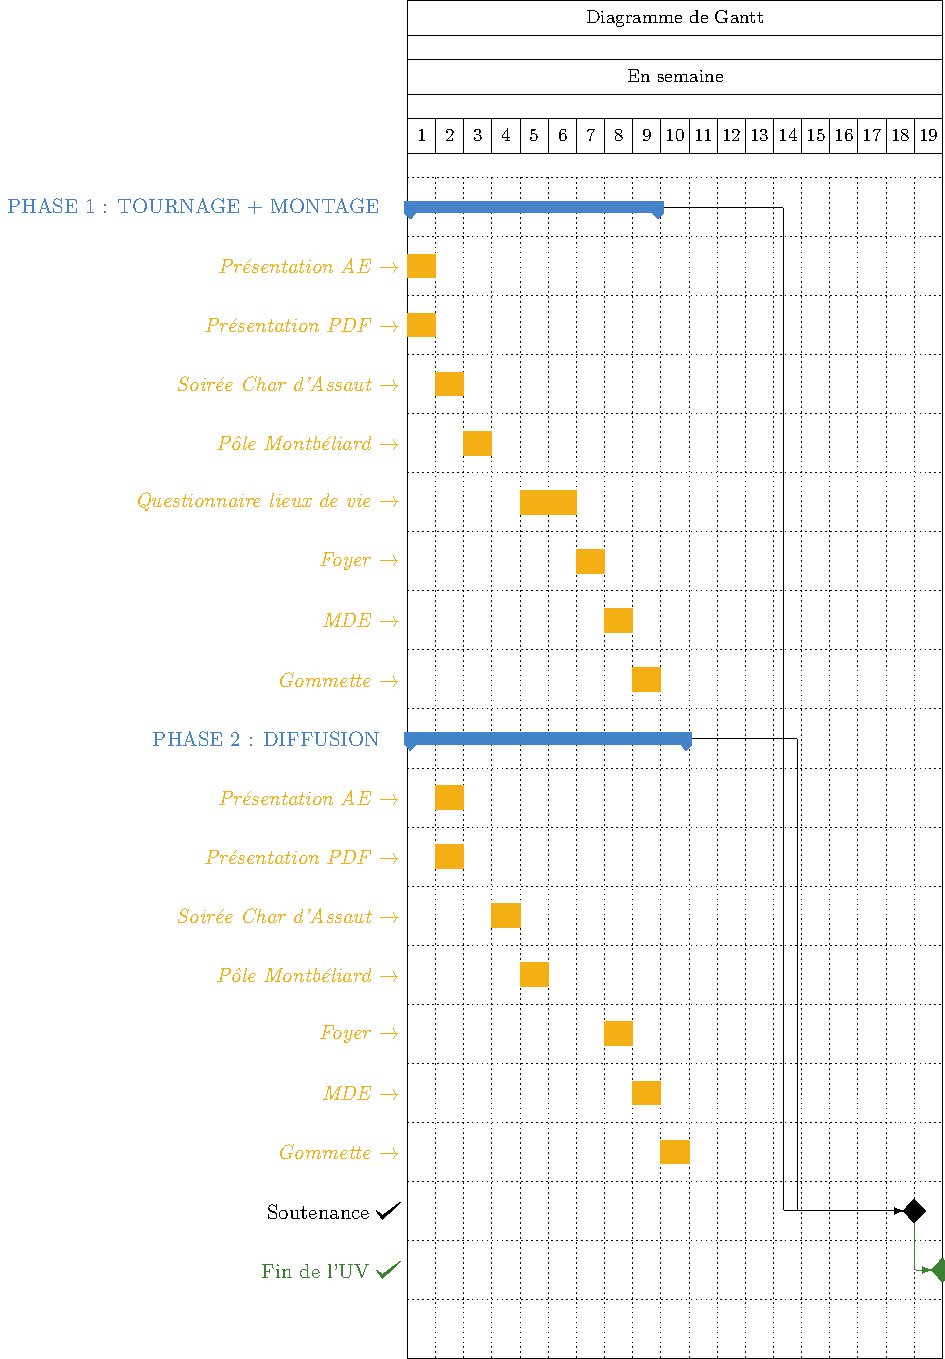
\includegraphics[scale=0.6]{ressources/gantt}
        \caption{Gantt initial \label{fig:ganttIni}}
    \end{center}
\end{figure}

L'objectif de ce projet est de réaliser rapidement des vidéos pour présenter l'association et les lieux de vie aux nouveaux·elles étudiant·e·s.
Ainsi, j'ai dû réaliser l'ensemble du tournage de ces vidéos en environ 9 semaines.

Comme dans tout projet, les délais sont sensibles aux changements.
J'ai rencontré quelques difficultés avec la prise de son, devant emprunter les micros du Crunch Lab, ce qui limitait la spontanéité des différents tournages.
En fin de projet, l'\gls{AE} a investi dans deux micros sans fil, facilitant la réalisation de ma dernière vidéo ainsi que d'autres projets par le responsable communication de l'\gls{AE}.

De plus, la vidéo sur la présentation du Pôle Montbéliard n'a pas été réalisée.
Après discussion avec le président de l'\gls{AE}, nous avons décidé de combiner la présentation de la Gommette et du Pôle Montbéliard pour éviter des répétitions entre les deux vidéos.

Malgré la suppression de la vidéo de présentation de Montbéliard et des retards d'une ou deux semaines sur la fin du projet, dus aux contraintes scolaires et personnelles des intervenants, une grande partie des objectifs a été atteinte.
